\documentclass[12pt]{article}
\usepackage[utf8]{inputenc}
\usepackage{lmodern}
\usepackage[margin=2.5cm]{geometry}
\usepackage{graphicx}


\title{Práctica 1}
\author{Fernando Cruz Pineda \\ Alexys Gómez Elizalde \\ Moisés Corpus García}
\date{}

\begin{document}
\maketitle

\section*{Ejercicios}

\begin{enumerate}
    \item Lee lo siguiente \texttt{https://www.evanjones.ca/software/threading-linus-msg.html} y comparte en máximo 4 líneas de computadora a qué se refiere Linus Torvalds con un contexto de ejecución y cómo se relaciona con la definición en la sección 1 de esta práctica.
    \item ¿Cuántos hilos tiene disponibles tu computadora? \\
      Ejecuta \texttt{Runtime.getRuntime().availableProcessors()}, si son más de uno en el equipo escriban el de cada uno.

      Número de hilos de Fernando Cruz: 8

      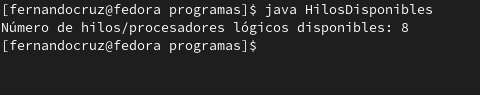
\includegraphics[]{Fer.png}

    \item Revisa el programa Determinante Concurrente y responde ¿Cuánto tiempo tarda en ejecutarse?

      Tiempo en equipo de Fernando: 1755939 ns

      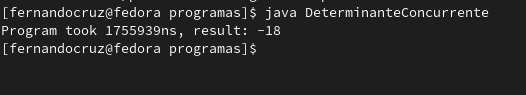
\includegraphics[]{Fer2.png}

      
    \item El programa Determinante Concurrente está implementado extendiendo la clase Thread. Implementa el programa utilizando la interfaz Runnable.

      Programa en programas/DeterminanteConcurrenteRunnable.java
      
    \item Implementa el programa Determinante Concurrente de forma secuencial.
      
      Programa en programas/DeterminanteSecuencial.java
      
    \item Implementa el programa Determinante Concurrente para dos hilos (en vez de seis).

      Programa en programas/DeterminanteDosHilos.java
      
    \item Compara las 3 implementaciones: el programa Determinante Concurrente para dos hilos, para seis hilos y el programa secuencial. Responde: ¿A qué se debe el orden en el que se ordenan los tiempos de ejecución de cada programa?
    \item Si utilizas la Ley de Amdahl entre el programa Determinante Concurrente para dos hilos y el programa secuencial. ¿El resultado es mayor o menor a 1? ¿Por qué?
    \item Describe con tus propias palabras en máximo dos líneas para qué sirve el método \texttt{join()}. Si no utilizas el método \texttt{join()} en Determinante Concurrente, ¿sigue funcionando?
\end{enumerate}

\end{document}
